% SECTION: Expectation-Maximization (EM) Algorithmus
\section{Expectation-Maximization (EM) Algorithmus}

\divider

% SUBSECTION: Problemstellung
\subsection{Problemstellung}

% Problemstellung
\begin{frame}{Problemstellung}{}
	\begin{itemize}
		\item Wir betrachten ein statistisches Modell mit Daten $\bX = \bigl( \bx_1, \bx_2, \ldots, \bx_N \bigr)^\top$, \keyword{latenten Variablen}
			$\bZ = \bigl( \bz_1, \bz_2, \ldots, \bz_N \bigr)^\top$ und Modellparametern $\btheta$.
		\item Unser Ziel ist die Maximierung der Log-Likelihood $\ln p(\bX; \btheta)$ bezüglich $\btheta$.
		\item Da wir die latenten Variablen nicht beobachten, müssen wir \textit{marginalisieren}:
		\begin{equation}
			\ln p(\bX; \btheta) = \ln \sum_{\bZ} p(\bX, \bZ; \btheta)
		\end{equation}
		\item In der Regel ist eine direkte Maximierung dieses Ausdrucks zu kompliziert,
			da der Logarithmus nicht direkt auf $p(\bX, \bZ; \btheta)$ wirken kann.
		\item Mit $\{ \bX, \bZ \}$ bezeichnen wir den \keyword{vollständigen} Datensatz, $\bX$ alleine nennen wir \keyword{unvollständig}.
			Analog nennen wir $\ln p(\bX, \bZ; \btheta)$ die \keyword{vollständige Log-Likelihood} und $\ln p(\bX; \btheta)$ die
			\keyword{unvollständige Log-Likelihood}.
	\end{itemize}
\end{frame}


% Expectation-Maximization (EM)
\begin{frame}{Expectation-Maximization (EM)}{}
	\begin{itemize}
		\item Da die Optimierung von $\ln p(\bX; \btheta)$ schwer ist, möchten wir also $\ln p(\bX, \bZ; \btheta)$ maximieren.
		\item \textbf{Problem:} Wir kennen $\bZ$ nicht.
		\item Der \keyword{Expectation-Maximization (EM) Algorithmus} löst dieses Problem iterativ in zwei Phasen,
			indem $\bZ$ in jeder Iteration bestmöglich geschätzt wird.
		\item Phasen:
		\begin{enumerate}
			\item \keyword{E-Phase:} Bestimme den Erwartungswert von $\ln p(\bX, \bZ; \btheta)$ unter der Aposteriori-Verteilung
				$p(\bZ \mid \bX; \bthetaOld)$. Die Erwartungswertfunktion bildet eine untere Schranke für $\ln p(\bX; \btheta)$.
			\item \keyword{M-Phase:} Die berechnete untere Schranke wird bezüglich der Parameter $\btheta$ maximiert,
				was zu den aktualisierten Parametern $\bthetaNew$ führt.
		\end{enumerate}
		\item Bei gegebenen Parametern $\bthetaOld$ erhält man so in jeder Iteration neue Parameter $\bthetaNew$,
			die zu einer höheren Log-Likelihood $\ln p(\bX; \btheta)$ führen.
	\end{itemize}
\end{frame}


% SUBSECTION: Ungleichung von Jensen
\subsection{Ungleichung von Jensen}

% Ungleichung von Jensen
\begin{frame}{Ungleichung von Jensen}{}
	Für unsere weiteren Betrachtungen benötigen wir die folgende Ungleichung:
	\begin{mytheo}[th:jensen]
		Es sei $X$ eine Zufallsvariable und $f$ eine \textit{konvexe} Funktion. Dann gilt die \keyword{Ungleichung von Jensen}
		(falls alle Erwartungswerte existieren)
		\begin{equation*}
			f\bigl( \E[X] \bigr) \le \E\bigl[ f(X) \bigr].
		\end{equation*}
	\end{mytheo}
	
	\textbf{Bemerkungen:}
	\begin{itemize}
		\item Für \textit{konkave} Funktionen $f$ gilt die Ungleichung in die andere Richtung: $f\bigl( \E[X] \bigr) \ge \E\bigl[ f(X) \bigr]$.
		\item Wenn $f$  \textit{strikt konvex} bzw. \textit{strikt konkav} ist, so gilt Gleichheit genau dann, wenn $X$ konstant (also nicht zufällig) ist.
	\end{itemize}
\end{frame}


% Visualisierung: Ungleichung von Jensen
\begin{frame}{Visualisierung: Ungleichung von Jensen}{}

\end{frame}


% SUBSECTION: Expectation-Schritt
\subsection{Expectation-Schritt}

% Bestimmung der unteren Schranke
\begin{frame}{Bestimmung der unteren Schranke}{}
	\begin{itemize}
		\item Im Folgenden konstruieren wir die oben erwähnte untere Schranke für $\ln p(\bX; \btheta)$.
		\item Hierzu führen wir die Verteilung $q$ über $\bZ$ mit $q(\bZ) \ne 0$ ein und erhalten
		\begin{align*}
			\ln p(\bX; \btheta)
				&= \ln \sum_{\bZ} p(\bX, \bZ; \btheta)
					= \ln \sum_{\bZ} q(\bZ) \cdot \frac{p(\bX, \bZ; \btheta)}{q(\bZ)}
		\\[2mm]
				&= \ln \E_{\bZ \sim q(\bZ)}\left[ \frac{p(\bX, \bZ; \btheta)}{q(\bZ)} \right]
		\\[2mm]
				&\ge \E_{\bZ \sim q(\bZ)} \left[ \ln \frac{p(\bX, \bZ; \btheta)}{q(\bZ)} \right] \eqqcolon \sL(q, \btheta).
		\end{align*}
		\item Für die Abschätzung im letzten Schritt haben wir die \keyword{Ungleichung von Jensen} (Satz \ref{th:jensen}) mit
			$f(x) \coloneqq \ln(x)$ (der Logarithmus ist strikt konkav) und $X \coloneqq \frac{p(\bX, \bZ; \btheta)}{q(\bZ)}$ benutzt.
	\end{itemize}
\end{frame}


% Bestimmung der unteren Schranke (Forts.)
\begin{frame}{Bestimmung der unteren Schranke (Forts.)}{}
	\begin{itemize}
		\item Die hergeleitete Ungleichung lässt sich mit den Logarithmengesetzen und der Linearität des Erwartungswerts umschreiben zu
		\begin{equation}
		\label{eq:em-untere-schranke}
			\ln p(\bX; \btheta) \ge \underbrace{
				\E_{\bZ \sim q(\bZ)}\left[ \ln p(\bX, \bZ; \btheta) \right]
			}_{\substack{\text{Erwartete vollständige} \\ \text{Log-Likelihood}}} - 
			\underbrace{
				\E_{\bZ \sim q(\bZ)}\left[ \ln q(\bZ) \right]
			}_{\text{Entropie von $q$}}.
		\end{equation}
		\item Die untere Schranke hängt von der Dichte $q$ ab, die wir noch bestimmen müsssen.
		\item Wir möchten $q$ so wählen, dass für das aktuelle $\btheta$ in \eqref{eq:em-untere-schranke} Gleichheit gilt.
		\item Die Ungleichung von Jensen (Satz \ref{th:jensen}) gilt mit Gleichheit, falls
		\begin{equation*}
			\frac{p(\bX, \bZ; \btheta)}{q(\bZ)} = \const.
		\end{equation*}
	\end{itemize}
\end{frame}


% Bestimmung der unteren Schranke (Forts.)
\begin{frame}{Bestimmung der unteren Schranke (Forts.)}{}
	\begin{itemize}
		\item Wegen der vorausgehenden Überlegungen müssen wir also $q(\bZ) \propto p(\bX, \bZ; \btheta)$ wählen. \\
			Das Symbol $\propto$ bedeutet \textit{proportional zu}.
		\item Daraus erhalten wir (da $q$ normiert sein muss)
		\begin{align*}
			q(\bZ)
				&= \frac{p(\bX, \bZ; \btheta)}{\sum_{\bZtilde} p(\bX, \bZtilde; \btheta)}
					= \frac{p(\bX, \bZ; \btheta)}{p(\bX; \btheta)}
		\\[2mm]
				&= p(\bZ \mid \bX; \btheta).
		\end{align*}
		\item \textbf{Ergebnis:} Für $q$ benutzen wir die Aposteriori-Verteilung von $\bZ$ gegeben $\bX$.
		\item Dies setzen wir in (\ref{eq:em-untere-schranke}) ein und erhalten die Identität
		\begin{equation*}
			\ln p(\bX; \btheta) = \E_{\bZ \sim p(\bZ \mid \bX; \btheta)}\left[ \ln p(\bX, \bZ; \btheta) \right]
				- \E_{\bZ \sim p(\bZ \mid \bX; \btheta)}\left[ \ln p(\bZ \mid \bX; \btheta) \right].
		\end{equation*}
	\end{itemize}
\end{frame}


% SUBSECTION: Maximization-Schritt
\subsection{Maximization-Schritt}

% Maximierung der unteren Schranke
\begin{frame}{Maximierung der unteren Schranke}{}
	\begin{itemize}
		\item Zu Beginn einer jeden EM-Iteration verfügen wir über den Parametervektor $\bthetaOld$, mit dem wir im E-Schritt
			die untere Schranke konstruieren.
		\item Hierbei wählen wir $q(\bZ) \coloneqq p\bigl( \bZ \mid \bX; \bthetaOld \bigr)$.
		\item Als untere Schranke erhalten wir damit
		\begin{align*}
			\ln p(\bX; \btheta)
				&\ge \E_{\bZ \sim p(\bZ \mid \bX; \bthetaOld)}\left[ \ln p\bigl( \bX, \bZ; \btheta \bigr) \right]
					- \E_{\bZ \sim p(\bZ \mid \bX; \bthetaOld)}\left[ \ln p\bigl( \bZ \mid \bX; \bthetaOld \bigr) \right]
		\\[2mm]
				&= Q\bigl( \btheta, \bthetaOld \bigr) + H\bigl( \bthetaOld, \bthetaOld \bigr)
		\\[2mm]
				&= Q\bigl( \btheta, \bthetaOld \bigr) + \const,
		\end{align*}
			wobei $Q$ der erste Erwartungswert und $H$ der negierte zweite Erwartungswert ist.
		\item Die Funktion $H\bigl( \bthetaOld, \bthetaOld \bigr)$ ist die \keyword{Entropie} von $\bthetaOld$.
	\end{itemize}
\end{frame}


% Maximierung der unteren Schranke (Forts.)
\begin{frame}{Maximierung der unteren Schranke (Forts.)}{}
	\begin{itemize}
		\item Da die Entropie $H\bigl( \bthetaOld, \bthetaOld \bigr)$ bezüglich $\btheta$ konstant ist, ist der im M-Schritt zu maximierende
			Ausdruck durch $Q\bigl( \btheta, \bthetaOld \bigr)$ gegeben.
		\item Der M-Schritt hat also die Form
		\begin{equation}
			\bthetaNew \coloneqq \argmax_{\btheta} Q\bigl( \btheta, \bthetaOld \bigr).
		\end{equation}
		\item Weiter unten beweisen wir noch, dass tatsächlich $p\bigl(\bX \mid \bthetaNew \bigr) \ge p\bigl(\bX \mid \bthetaOld \bigr)$ gilt.
		\item Zunächst fassen wir den EM-Algorithmus übersichtlich zusammen.
	\end{itemize}
\end{frame}


% SUBSECTION: EM-Algorithmus und Konvergenz
\subsection{EM-Algorithmus und Konvergenz}

% EM-Algorithmus
\begin{frame}{EM-Algorithmus}{}
	\begin{myalg}
		\begin{enumerate}
			\item Initialisiere $\bthetaOld$.
			\item \textbf{E-Schritt:} Bestimme die untere Schranke
			\begin{equation*}
				Q\bigl( \btheta, \bthetaOld \bigr) \coloneqq \E_{\bZ \sim p(\bZ \mid \bX; \bthetaOld)}\left[ \ln p(\bX, \bZ; \btheta) \right].
			\end{equation*}
			\item \textbf{M-Schritt:} Maximiere die untere Schranke und berechne
			\begin{equation*}
				\bthetaNew \coloneqq \argmax_{\btheta} Q\bigl( \btheta, \bthetaOld \bigr).
			\end{equation*}
			\item Falls noch nicht konvergiert, gehe zurück zu Schritt 2 und setze $\bthetaOld \coloneqq \bthetaNew$.
			\item Ansonsten gebe $\bthetaNew$ zurück.
		\end{enumerate}
	\end{myalg}
\end{frame}


% Konvergenz des EM-Algorithmus
\begin{frame}{Konvergenz des EM-Algorithmus}{}
	\begin{itemize}
		\item Zum Abschluss beweisen wir noch die Konvergenz des EM-Algorithmus.
		\item Es gilt
		\begin{align*}
			\ln p\bigl( \bX; \bthetaNew \bigr)
				&\ge \sum_{\bZ} p\bigl( \bZ \mid \bX; \bthetaOld \bigr)
					\ln \frac{p\bigl( \bX, \bZ; \bthetaNew \bigr)}{p\bigl( \bZ \mid \bX; \bthetaOld \bigr)}
		\\[2mm]
				&\ge \sum_{\bZ} p\bigl( \bZ \mid \bX; \bthetaOld \bigr)
					\ln \frac{p\bigl( \bX, \bZ; \bthetaOld \bigr)}{p\bigl( \bZ \mid \bX; \bthetaOld \bigr)}
		\\[2mm]
				&= \ln p\bigl( \bX; \bthetaOld \bigr).
		\end{align*}
		\item Die erste Ungleichung gilt hierbei aufgrund der Definition der unteren Schranke.
		\item Die zweite Ungleichung gilt, weil $\bthetaNew$ so gewählt wurde, dass es die untere Schranke maximiert.
	\end{itemize}
\end{frame}


% Visualisierung: EM-Algorithmus
\begin{frame}{Visualisierung: EM-Algorithmus}{}
	\begin{figure}
		\centering
		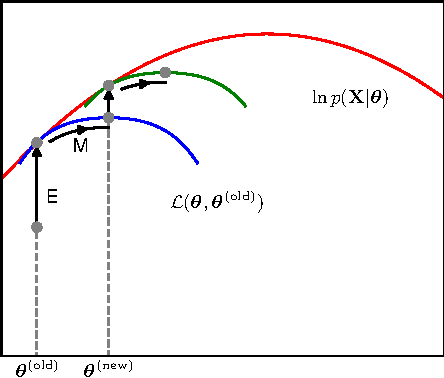
\includegraphics[scale=0.75]{./img/em/em_visual}
		\caption{Veranschaulichung des EM-Algorithmus. Siehe \cite{Bishop2024}, Seite 488.}
	\end{figure}
\end{frame}


% SUBSECTION: Evidence-Lower-Bound und Kullback-Leibler Divergenz
\subsection{Evidence-Lower-Bound und Kullback-Leibler Divergenz}

% Eine andere Sicht auf den EM-Algorithmus
\begin{frame}{Eine andere Sicht auf den EM-Algorithmus}{}
	\begin{itemize}
		\item Die Log-Likelihood $\ln p(\bX; \btheta)$ können wir zerlegen in
		\begin{equation}
		\label{eq:zerlegung-unvollst-logl}
			\ln p(\bX; \btheta) = \sL(q, \btheta) + \KL(q \parallel p).
		\end{equation}
		\item Dabei ist:
		\begin{itemize}
			\item $\sL(q, \btheta)$ die \keyword{Evidence Lower Bound (ELBO)} oder auch \keyword{Variational Lower Bound} mit
			\begin{equation}
			\label{eq:elbo}
				\sL(q, \btheta)
					\coloneqq \sum_{\bZ} q(\bZ) \ln \frac{p(\bX, \bZ; \btheta)}{q(\bZ)}
					= \sum_{\bZ} q(\bZ) \cdot \bigl[ \ln p(\bX, \bZ; \btheta) - \ln q(\bZ) \bigr].
			\end{equation}
			\item $\KL(q \parallel p)$ die \keyword{Kullback-Leibler Divergenz} zwischen $q(\bZ)$ und $p(\bZ \mid \bX; \btheta)$, welche gegeben ist durch
			\begin{equation}
				\KL(q \parallel p)
					\coloneqq -\sum_{\bZ} q(\bZ) \ln \frac{p(\bZ \mid \bX; \btheta)}{q(\bZ)}
					= -\sum_{\bZ} q(\bZ) \cdot \bigl[ \ln p(\bZ \mid \bX; \btheta) - \ln q(\bZ) \bigr].
			\end{equation}
		\end{itemize}
	\end{itemize}
\end{frame}


% Beweis der Zerlegung \eqref{eq:zerlegung-unvollst-logl}
\begin{frame}{Beweis der Zerlegung \eqref{eq:zerlegung-unvollst-logl}}{}
	\begin{myproof}
		Wir beweisen die Zerlegung \eqref{eq:zerlegung-unvollst-logl}. Hierzu wenden wir die Kettenregel für Wahrscheinlichkeiten auf $p(\bX, \bZ; \btheta)$
		an. Wir erhalten $p(\bX, \bZ; \btheta) = p(\bZ \mid \bX; \btheta) \cdot p(\bX; \btheta)$. Anwendung des Logarithmus ergibt
		$$\ln p(\bX, \bZ; \btheta) = \ln p(\bZ \mid \bX; \btheta) + \ln p(\bX; \btheta).$$ Dies setzen wir in die Evidence Lower Bound \eqref{eq:elbo} ein
		und erhalten
		\begin{align*}
			\sL(q, \btheta)
				&= \sum_{\bZ} q(\bZ) \cdot \bigl[ \ln p(\bX, \bZ; \btheta) - \ln q(\bZ) \bigr]
		\\[2mm]
				&= \sum_{\bZ} q(\bZ) \cdot \bigl[ \ln p(\bZ \mid \bX; \btheta) + \ln p(\bX; \btheta) - \ln q(\bZ) \bigr].
		\end{align*}
		Damit erhalten wir schließlich
		\begin{align*}
			\sL(q, \btheta) + \KL(q \parallel p)
				&= \sum_{\bZ} q(\bZ) \cdot \bigl[ \ln p(\bZ \mid \bX; \btheta) + \ln p(\bX; \btheta) - \ln q(\bZ) \bigr]
					- \sum_{\bZ} q(\bZ) \cdot \bigl[ \ln p(\bZ \mid \bX; \btheta) - \ln q(\bZ) \bigr]
		\\[2mm]
				&= \sum_{\bZ} q(\bZ) \cdot \ln p(\bX; \btheta) = \ln p(\bX; \btheta) \cdot \sum_{\bZ} q(\bZ) = \ln p(\bX; \btheta).
		\end{align*}
	\end{myproof}
\end{frame}


% Visualisierung: Zerlegung der Log-Likelihood
\begin{frame}{Visualisierung: Zerlegung der Log-Likelihood}{}
	\begin{figure}
		\centering
		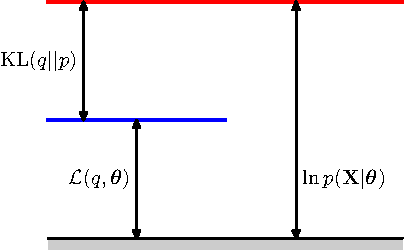
\includegraphics[scale=1.00]{./img/em/em_decomposition_log_likelihood}
		\caption{Veranschaulichung der Zerlegung \eqref{eq:zerlegung-unvollst-logl}. Siehe \cite{Bishop2024}, Seite 486.}
	\end{figure}
\end{frame}